\documentclass[12pt, titlepage]{article}

\usepackage{fullpage}
\usepackage[round]{natbib}
\usepackage{multirow}
\usepackage{booktabs}
\usepackage{tabularx}
\usepackage{graphicx}
\usepackage{float}
\usepackage{hyperref}
\hypersetup{
    colorlinks,
    citecolor=blue,
    filecolor=black,
    linkcolor=red,
    urlcolor=blue
}

%% Comments

\usepackage{color}

\newif\ifcomments\commentstrue %displays comments
%\newif\ifcomments\commentsfalse %so that comments do not display

\ifcomments
\newcommand{\authornote}[3]{\textcolor{#1}{[#3 ---#2]}}
\newcommand{\todo}[1]{\textcolor{red}{[TODO: #1]}}
\else
\newcommand{\authornote}[3]{}
\newcommand{\todo}[1]{}
\fi

\newcommand{\wss}[1]{\authornote{blue}{SS}{#1}} 
\newcommand{\plt}[1]{\authornote{magenta}{TPLT}{#1}} %For explanation of the template
\newcommand{\an}[1]{\authornote{cyan}{Author}{#1}}

%% Common Parts

\newcommand{\progname}{ProgName} % PUT YOUR PROGRAM NAME HERE
\newcommand{\authname}{Team \#, Team Name
\\ Student 1 name
\\ Student 2 name
\\ Student 3 name
\\ Student 4 name} % AUTHOR NAMES                  

\usepackage{hyperref}
    \hypersetup{colorlinks=true, linkcolor=blue, citecolor=blue, filecolor=blue,
                urlcolor=blue, unicode=false}
    \urlstyle{same}
                                


\newcounter{acnum}
\newcommand{\actheacnum}{AC\theacnum}
\newcommand{\acref}[1]{AC\ref{#1}}

\newcounter{ucnum}
\newcommand{\uctheucnum}{UC\theucnum}
\newcommand{\uref}[1]{UC\ref{#1}}

\newcounter{mnum}
\newcommand{\mthemnum}{M\themnum}
\newcommand{\mref}[1]{M\ref{#1}}

\begin{document}

\title{Module Guide for Centrality in Graphs} 
\author{Atiyeh Sayadi}
\date{\today}

\maketitle

\pagenumbering{roman}

\section{Revision History}

\begin{tabularx}{\textwidth}{p{3cm}p{2cm}X}
\toprule {\bf Date} & {\bf Version} & {\bf Notes}\\
\midrule
March 12, 2024 & 1.0 & Initial draft\\
\bottomrule
\end{tabularx}

\newpage

\section{Reference Material}

This section records information for easy reference.

\subsection{Abbreviations and Acronyms}

\renewcommand{\arraystretch}{1.2}
\begin{tabular}{l l} 
  \toprule		
  \textbf{symbol} & \textbf{description}\\
  \midrule 
  AC & Anticipated Change\\
CC & Closeness Centrality\\
  CIG& Centrality in Graphs\\
  DAG & Directed Acyclic Graph \\
DC & Degree Centrality\\
  M & Module \\
  MG & Module Guide \\
  OS & Operating System \\
  R & Requirement\\
  SC & Scientific Computing \\
  SRS & Software Requirements Specification\\
  UC & Unlikely Change \\
  \bottomrule
\end{tabular}\\

\newpage

\tableofcontents

\listoftables

\listoffigures

\newpage

\pagenumbering{arabic}

\section{Introduction}

Decomposing a system into modules is a commonly accepted approach to developing
software.  A module is a work assignment for a programmer or programming
team~\citep{ParnasEtAl1984}.  We advocate a decomposition
based on the principle of information hiding~\citep{Parnas1972a}.  This
principle supports design for change, because the ``secrets'' that each module
hides represent likely future changes.  Design for change is valuable in SC,
where modifications are frequent, especially during initial development as the
solution space is explored.  

Our design follows the rules layed out by \citet{ParnasEtAl1984}, as follows:
\begin{itemize}
\item System details that are likely to change independently should be the
  secrets of separate modules.
\item Each data structure is implemented in only one module.
\item Any other program that requires information stored in a module's data
  structures must obtain it by calling access programs belonging to that module.
\end{itemize}

After completing the first stage of the design, the Software Requirements
Specification (SRS), the Module Guide (MG) is developed~\citep{ParnasEtAl1984}. The MG
specifies the modular structure of the system and is intended to allow both
designers and maintainers to easily identify the parts of the software.  The
potential readers of this document are as follows:

\begin{itemize}
\item New project members: This document can be a guide for a new project member
  to easily understand the overall structure and quickly find the
  relevant modules they are searching for.
\item Maintainers: The hierarchical structure of the module guide improves the
  maintainers' understanding when they need to make changes to the system. It is
  important for a maintainer to update the relevant sections of the document
  after changes have been made.
\item Designers: Once the module guide has been written, it can be used to
  check for consistency, feasibility, and flexibility. Designers can verify the
  system in various ways, such as consistency among modules, feasibility of the
  decomposition, and flexibility of the design.
\end{itemize}

The rest of the document is organized as follows. Section
\ref{SecChange} lists the anticipated and unlikely changes of the software
requirements. Section \ref{SecMH} summarizes the module decomposition that
was constructed according to the likely changes. Section \ref{SecConnection}
specifies the connections between the software requirements and the
modules. Section \ref{SecMD} gives a detailed description of the
modules. Section \ref{SecTM} includes two traceability matrices. One checks
the completeness of the design against the requirements provided in the SRS. The
other shows the relation between anticipated changes and the modules. Section
\ref{SecUse} describes the use relation between modules.

\section{Anticipated and Unlikely Changes} \label{SecChange}

This section lists possible changes to the system. According to the likeliness
of the change, the possible changes are classified into two
categories. Anticipated changes are listed in Section \ref{SecAchange}, and
unlikely changes are listed in Section \ref{SecUchange}.

\subsection{Anticipated Changes} \label{SecAchange}

This software, like other softwares, may undergo changes. These changes are as follows:

\begin{description}
\item[\refstepcounter{acnum} \actheacnum \label{acHardware}:] Changing the Initial Graph from Undirected to Directed.
\item[\refstepcounter{acnum} \actheacnum \label{acInput}:] Computing Other Centrality Measures such as Betweenness Centrality.
\item[\refstepcounter{acnum} \actheacnum \label{computation}:]  Reading a file from various inputs such as Excel.
\end{description}

\subsection{Unlikely Changes} \label{SecUchange}

The future changes of the software do not include the following items:

\begin{description}
\item[\refstepcounter{ucnum} \uctheucnum \label{ucIO}:] The input matrix will still be of size n*2.
\item[\refstepcounter{ucnum} \uctheucnum \label{measure}:] The graph representation in the output will remain unchanged. A visual depiction of the graph will still be displayed.
\end{description}

\section{Module Hierarchy} \label{SecMH}

This section provides an overview of the module design. Modules are summarized
in a hierarchy decomposed by secrets in Table \ref{TblMH}. The modules listed
below, which are leaves in the hierarchy tree, are the modules that will
actually be implemented.

\begin{description}
\item [\refstepcounter{mnum} \mthemnum \label{mHH}:] Hardware-Hiding Module
\item [\refstepcounter{mnum} \mthemnum \label{mHH}:] Behaviour-Hiding Module
\item [\refstepcounter{mnum} \mthemnum \label{mHH}:] Software Decision Module
\end{description}


\begin{table}[h!]
\centering
\begin{tabular}{p{0.3\textwidth} p{0.6\textwidth}}
\toprule
\textbf{Level 1} & \textbf{Level 2}\\
\midrule

{Hardware-Hiding Module} & - \\
\midrule

{Behaviour-Hiding Module} & Show Graph\\ & File\\ & Graph\\
\midrule

\multirow{3}{0.3\textwidth}{Software Decision Module} & Matrix\\ & GUI Provider\\
\bottomrule

\end{tabular}
\caption{Module Hierarchy}
\label{TblMH}
\end{table}

\section{Connection Between Requirements and Design} \label{SecConnection}

The design of the system is intended to satisfy the requirements developed in
the SRS. In this stage, the system is decomposed into modules. The connection
between requirements and modules is listed in Table~\ref{TblRT}.\\\\
\textbf{Functional requirments:}
\begin{description}
\item FR1: Degree centrality for all nodes ranges between zero and one.
\item FR2: Degree centrality has been calculated for all nodes.
\item FR3: Closeness centrality for all nodes ranges between zero and one.
\item FR4: Closeness centrality has been calculated for all nodes.\\
\end{description}

\textbf{Nonfunctional requirments:}
\begin{description}
\item NFR1: Accuracy
\item NFR2: Usability
\item NFR3: Maintainability
\end{description}


\section{Module Decomposition} \label{SecMD}

Modules are decomposed according to the principle of ``information hiding''
proposed by \citet{ParnasEtAl1984}. 
The following is an introduction to the modules and a brief explanation of each of them.


\subsection{Hardware Hiding Modules }
\begin{description}
\item[Secrets:]The data structure and algorithm used to implement the virtual
  hardware.
\item[Services:]Serves as a virtual hardware used by the rest of the
 system. This module provides the interface between the hardware and the
 software. So, the system can use it to display outputs or to accept inputs.
\item[Implemented By:] OS
\end{description}
\subsection{Behaviour-Hiding Module}



\subsubsection{File }

\begin{description}
\item[Secrets:] The file format.
\item[Services:] This module reads the initial file containing graph data from the input and returns the obtained graph using Graph module in the output.
\item[Implemented By:] CIG
\item[Type of Module:] Record
\end{description}

\subsubsection{Show Graph }
\begin{description}
\item[Secrets:] Setting up user interface settings for displaying outputs.
\item[Services:] This module generates output for both centrality measures, degree centrality and betweenness centrality, on the initial graph.
\item[Implemented By:] CIG
\item[Type of Module:] Abstract data type
\end{description}

\subsubsection{Graph }
\begin{description}
\item[Secrets:] Data structure for a graph using the concept of adjacency matrix and computational algorithms for graphs.
\item[Services:] This module provides a data structure for a graph, which consists of a set of nodes and edges. Then, based on this information, it calculates the node degree, the shortest path from one node to other nodes, degree centrality, and closeness centrality.
\item[Implemented By:] CIG
\item[Type of Module:] Abstract data type
\end{description}


\subsection{Software Decision Module}

\subsubsection{Matrix}
\begin{description}
\item[Secrets:] A module for performing mathematical calculations on multi-dimensional data.
\item[Services:] Using the NumPy library, operations on matrices, such as creating matrices, loading them, calculating their size, etc., can be performed as follows.
  % Changes in these modules are more likely to be motivated by a desire to
  % improve performance than by externally imposed changes.
\item[Implemented By:] Numpy
\item[Type of Module:] Library
\end{description}

\subsubsection{GUI Provider}
\begin{description}
\item[Secrets:] Providing a graphical user interface.
\item[Services:] Using the Tkinter library and its functions in Python to create a graphical user interface (GUI).
  % Changes in these modules are more likely to be motivated by a desire to
  % improve performance than by externally imposed changes.
\item[Implemented By:] Tkinter
\item[Type of Module:] Library
\end{description}
\section{Traceability Matrix} \label{SecTM}

This section shows two traceability matrices: between the modules and the
requirements and between the modules and the anticipated changes.

% the table should use mref, the requirements should be named, use something
% like fref
\begin{table}[H]
\centering
\begin{tabular}{p{0.2\textwidth} p{0.6\textwidth}}
\toprule
\textbf{Req.} & \textbf{Modules}\\
\midrule
FR1 & Graph \\
FR2 & Graph\\
FR3 & Graph\\
FR4 & Graph\\
NFR1 & Graph, File, GUI Provider, Matrix, Show Graph\\
NFR2 & Graph, File, GUI Provider, Matrix, Show Graph\\
NFR3 & Graph, File, GUI Provider, Matrix, Show Graph\\
\bottomrule
\end{tabular}
\caption{Trace Between Requirements and Modules}
\label{TblRT}
\end{table}

\begin{table}[H]
\centering
\begin{tabular}{p{0.2\textwidth} p{0.6\textwidth}}
\toprule
\textbf{AC} & \textbf{Modules}\\
\midrule
AC1 & Graph\\
AC2 &Graph, Show Graph\\
AC3 & File\\
\bottomrule
\end{tabular}
\caption{Trace Between Anticipated Changes and Modules}
\label{TblACT}
\end{table}

\section{Use Hierarchy Between Modules} \label{SecUse}

Figure 1 illustrates a hierarchical view of the relationship between the modules.
\begin{figure}[h!]
\begin{center}
 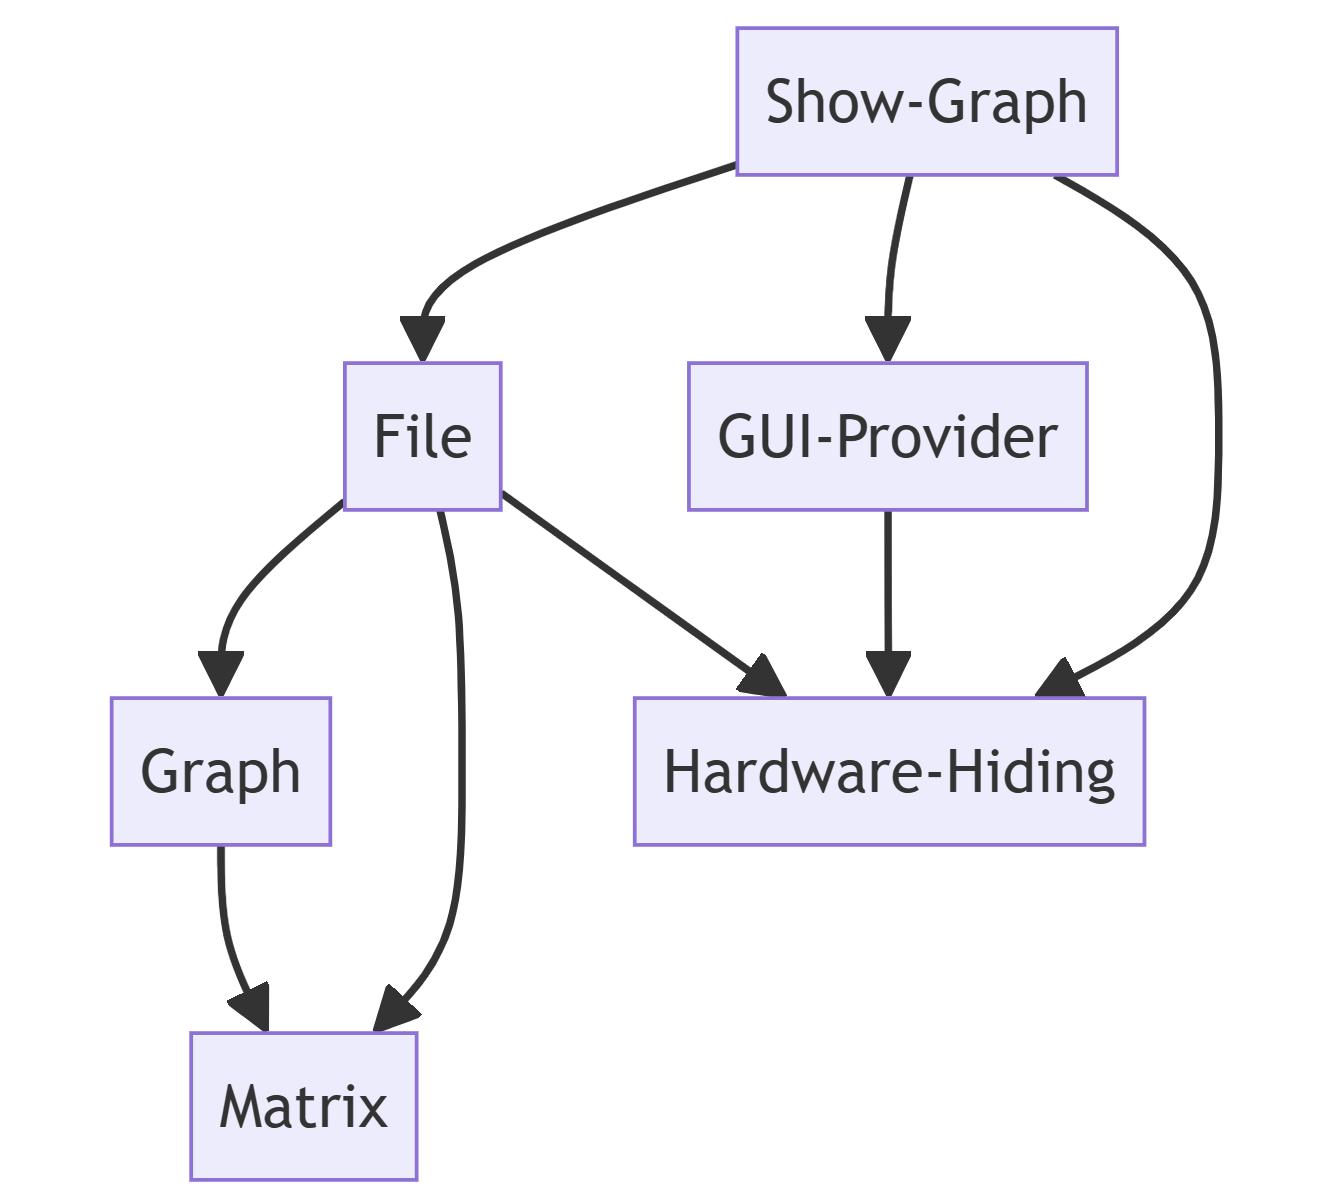
\includegraphics[width=0.6\textwidth]{GRAPH}
\caption{Use hierarchy among modules}
\label{Fig_SystemContext} 
\end{center}
\end{figure}

\section{User Interfaces}

This software provides a simple graphical interface that displays the graph image for both centrality measures, degree centrality and closeness centrality, while indicating the respective values for each node.

\section{Design of Communication Protocols}

\section{Timeline}


Table 4 displays the timeline for the development of each module and its respective developer.

\begin{table}[H]
\centering
\begin{tabular}{p{0.2\textwidth} p{0.4\textwidth}  p{0.4\textwidth}}
\toprule
 \textbf{Modules} & \textbf{Time} & \textbf{Responsible} \\
\midrule
File& 20-25 March& Atiyeh Sayadi\\
Graph & 12-20 March& Atiyeh Sayadi\\
Show Graph & 25-29 April& Atiyeh Sayadi\\
\bottomrule
\end{tabular}
\caption{Timeline}
\end{table}

\bibliographystyle {plainnat}
\bibliography{../../../refs/References}

\newpage{}

\end{document}